\begin{figure*}[width=2\columnwidth]
	\centering
	\subfloat[No Tactic]{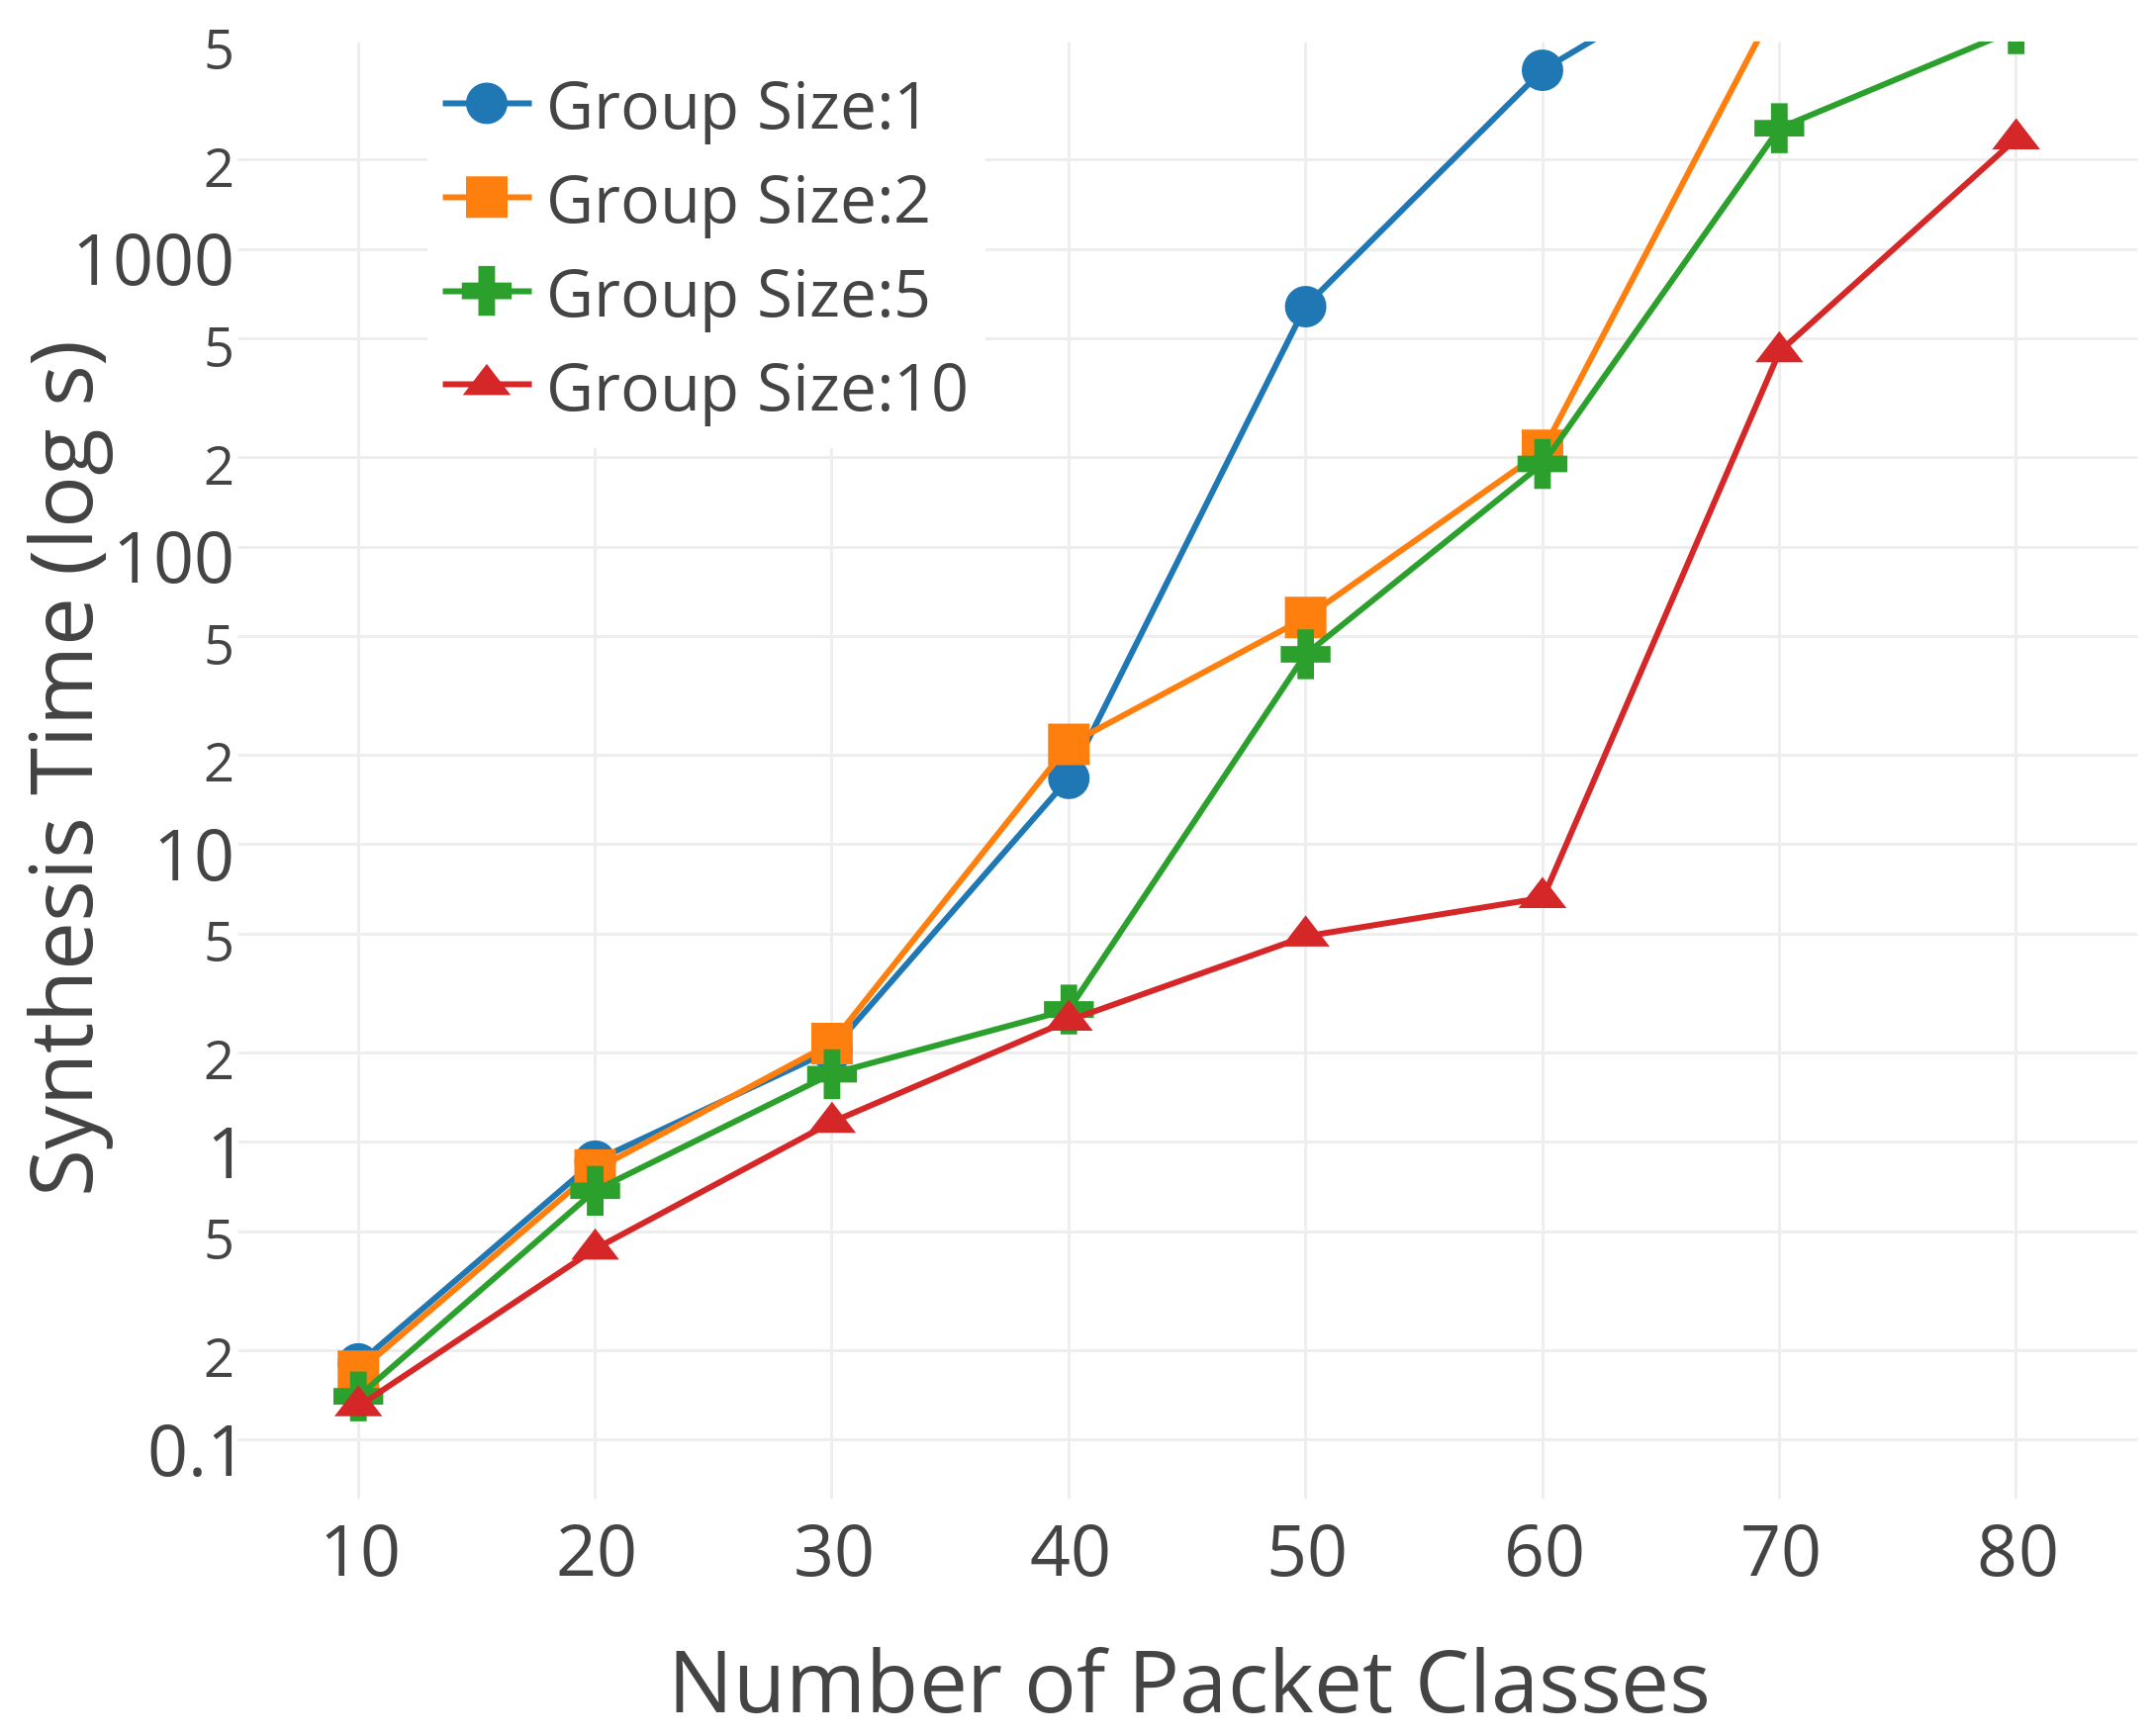
\includegraphics[width=0.66\columnwidth]{figures/no-tactic-isolation-plot.eps}}
	\subfloat[No Edge Tactic]{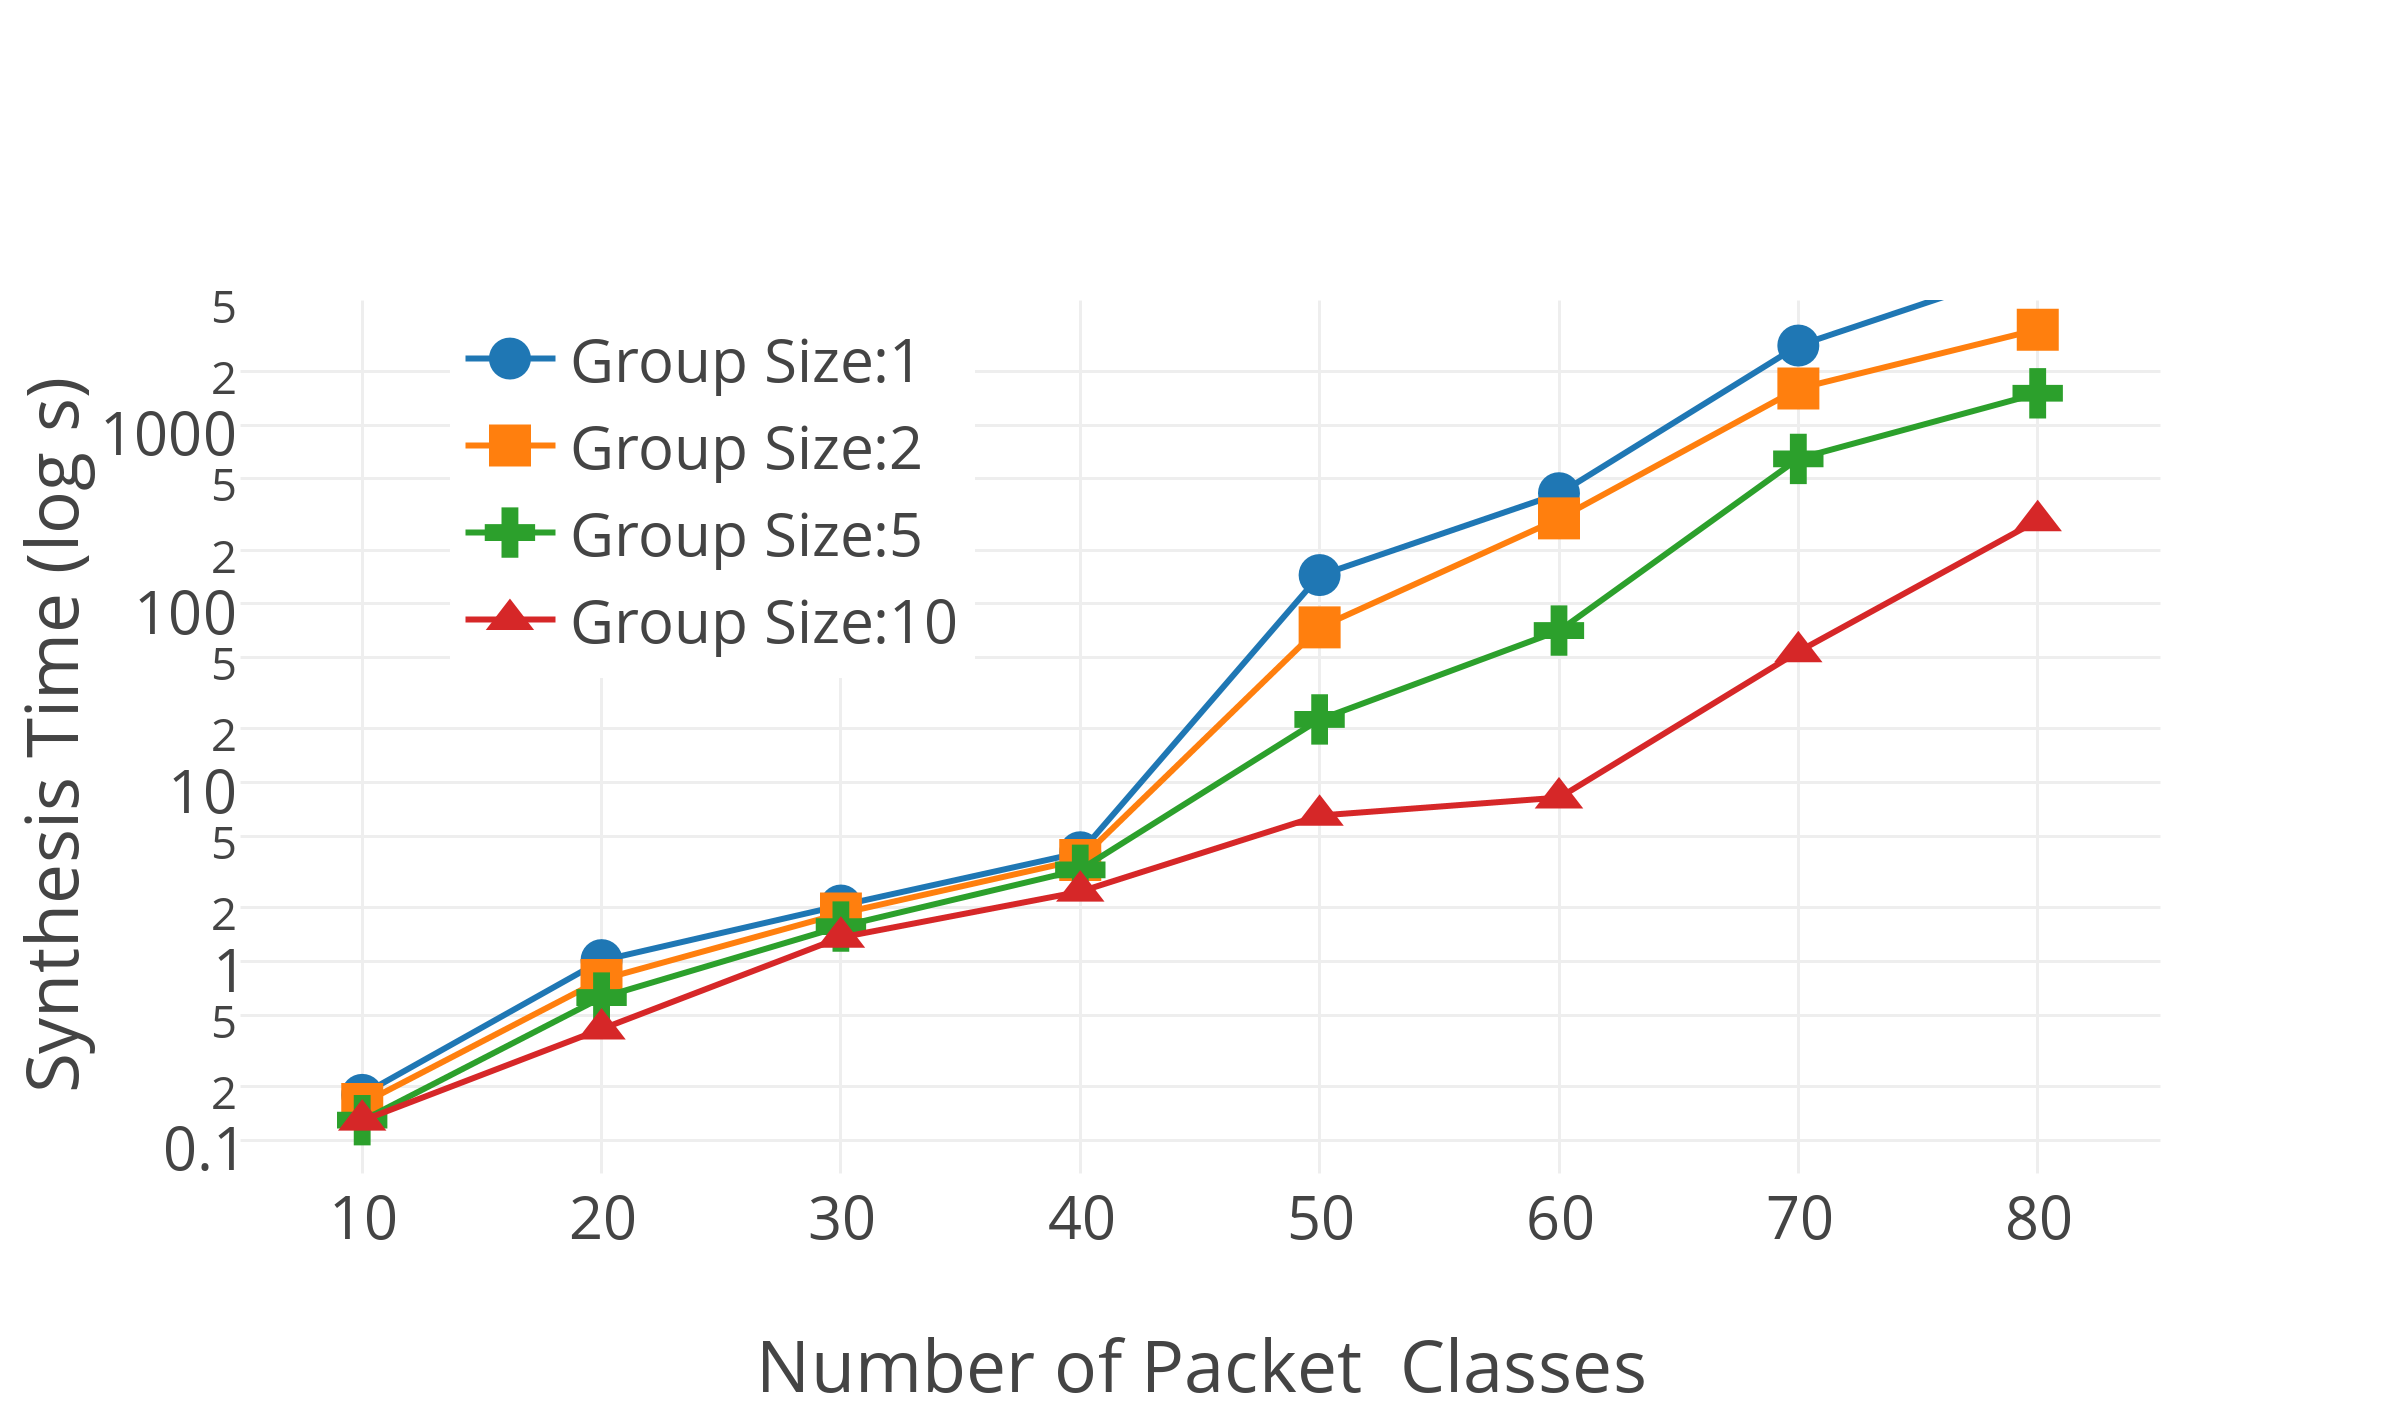
\includegraphics[width=0.66\columnwidth]{figures/no-edge-tactic-isolation-plot.eps}}
	\subfloat[Valley-free Routing Tactic]{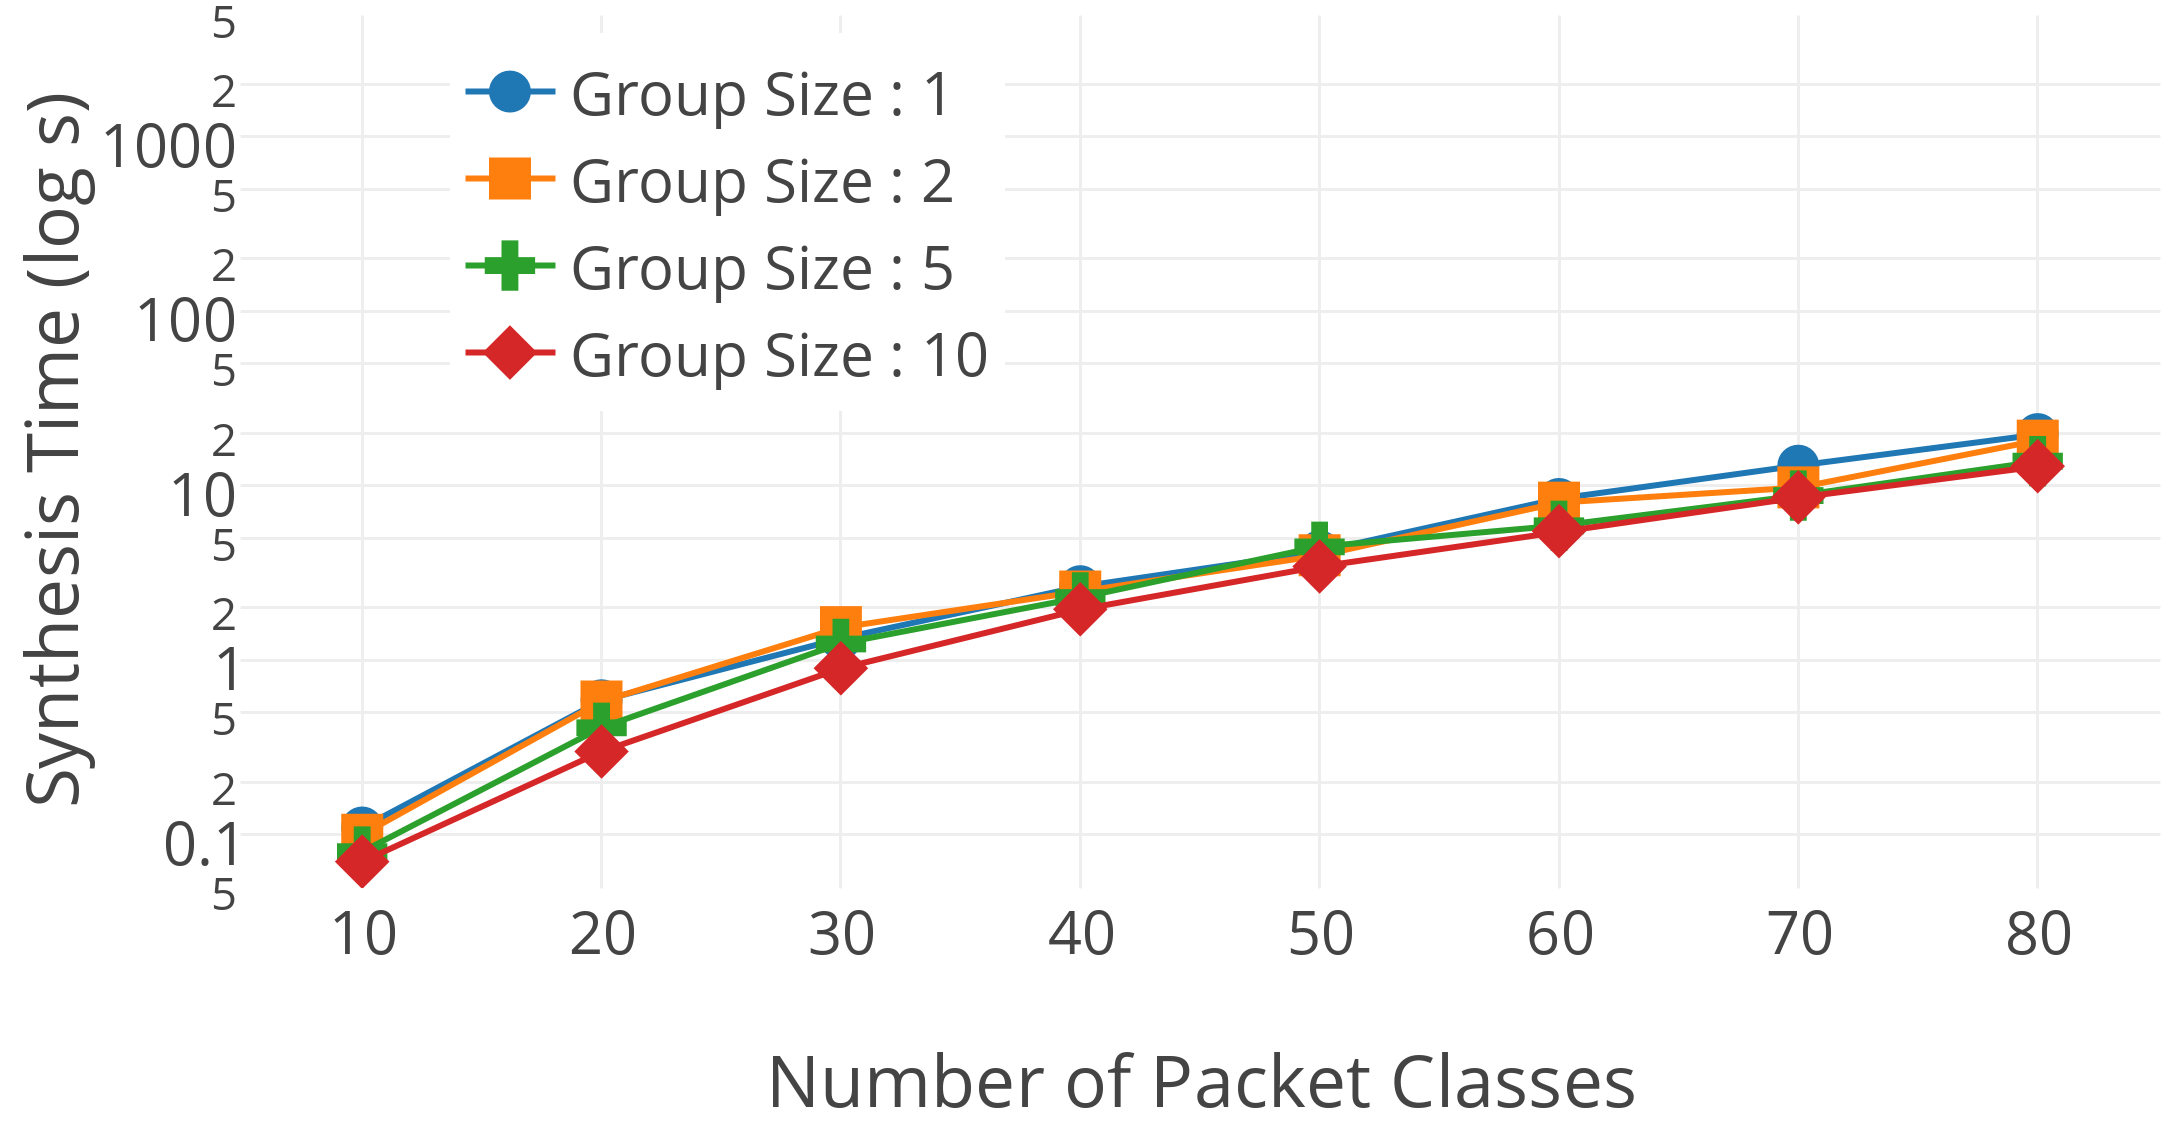
\includegraphics[width=0.66\columnwidth]{figures/eacae-isolation-plot.eps}}
	\caption{\label{fig:isolation}
		Total synthesis time (log scale) for isolation workloads over range of packet classes and different tenant-group sizes.}
\end{figure*}

\section{Evaluation}
In this section, we evaluate \Name using realistic multi-tenant data
center settings. Specifically, we ask:

\begin{itemize}

\item What is the performance of \Name's baseline synthesis
  algorithms? How does the performance vary with the size of the
  network, number of policies, and the nature of policies in use?

\item To what extent do tactic help improve \Name's synthesis
  performance? Which tactics offer the best improvement?

\item To what extent does optimistic synthesis improve \Name's
  performance? When does it lead to degraded synthesis times?

\item what else? XXX

\end{itemize}

In our evaluation, we target enterprise-scale could data centers. In
particular, the settings we study have a few thousand servers, tens of
switches, and hierarchical fat-tree like network topologies. At the
most basic level, our experiments are parameterized by: (a) total size
of the network which we vary between 45 to 180 switches, (b) number of
tenants (1-80), (c) number of packet classes in a tenant (1-10). 

Our primary metric of interest is synthesis time, measured in
seconds. In measuring this, we focus on the time the Z3 solver takes
to solve the constraints. All experiments were conducted using a
single (Cloudlab) machine with 32-core Intel-Xeon 2.40GHz CPU and
128GB of RAM.

% TODO : Write about max path length.

\subsection{Baseline Performance}
For evaluate the baseline performance of \Name without tactics, we model a multi-tenant
80-node fat-tree topology network with   
tenant-isolation in in \cref{fig:isolation}(a). 
For each workload, we have $n$ tenants with group size $g$ which 
is the number of packet classes for each tenant. The x-axis shows the total packet classes $n*g$. 
A single tenant's packet classes are not isolated to one another and isolated to all packet
classes belonging to other tenants. Thus, two tenants do not share a link, and can never affect
each other's performance. For empirical purposes, 
we randomly
\footnote{Smarter placement of tenants could speed-up synthesis as tenant endpoints would
	be located closer to each other. The placement algorithm can be used to develop specialised tactics.}
  place endpoints for the tenants' packet classes, ensuring that not more than 4 tenants share a single endpoint
  (each edge switch has $pod\_size/2 = 4$ links). 
   Operators can aggregate a tenant's traffic from one rack to
another to a single reachability policy and establish pathways for communication amongst the multiple
machines in different racks. 

For a fixed group size, we can observe that as number of packet classes increases,
the total synthesis time increases expotentially as expected (linearly in log scale). As we decrease group size,
 we can observe that synthesis time increases greatly for the same number of packet classes.
 As the number of tenants increases, consequently the problem is more constrainted 
  due to increased number of isolation policies. 
 Group size = 1 denotes the extreme case where all flows are isolated to one other. 
      
%\begin{figure}[H]
%	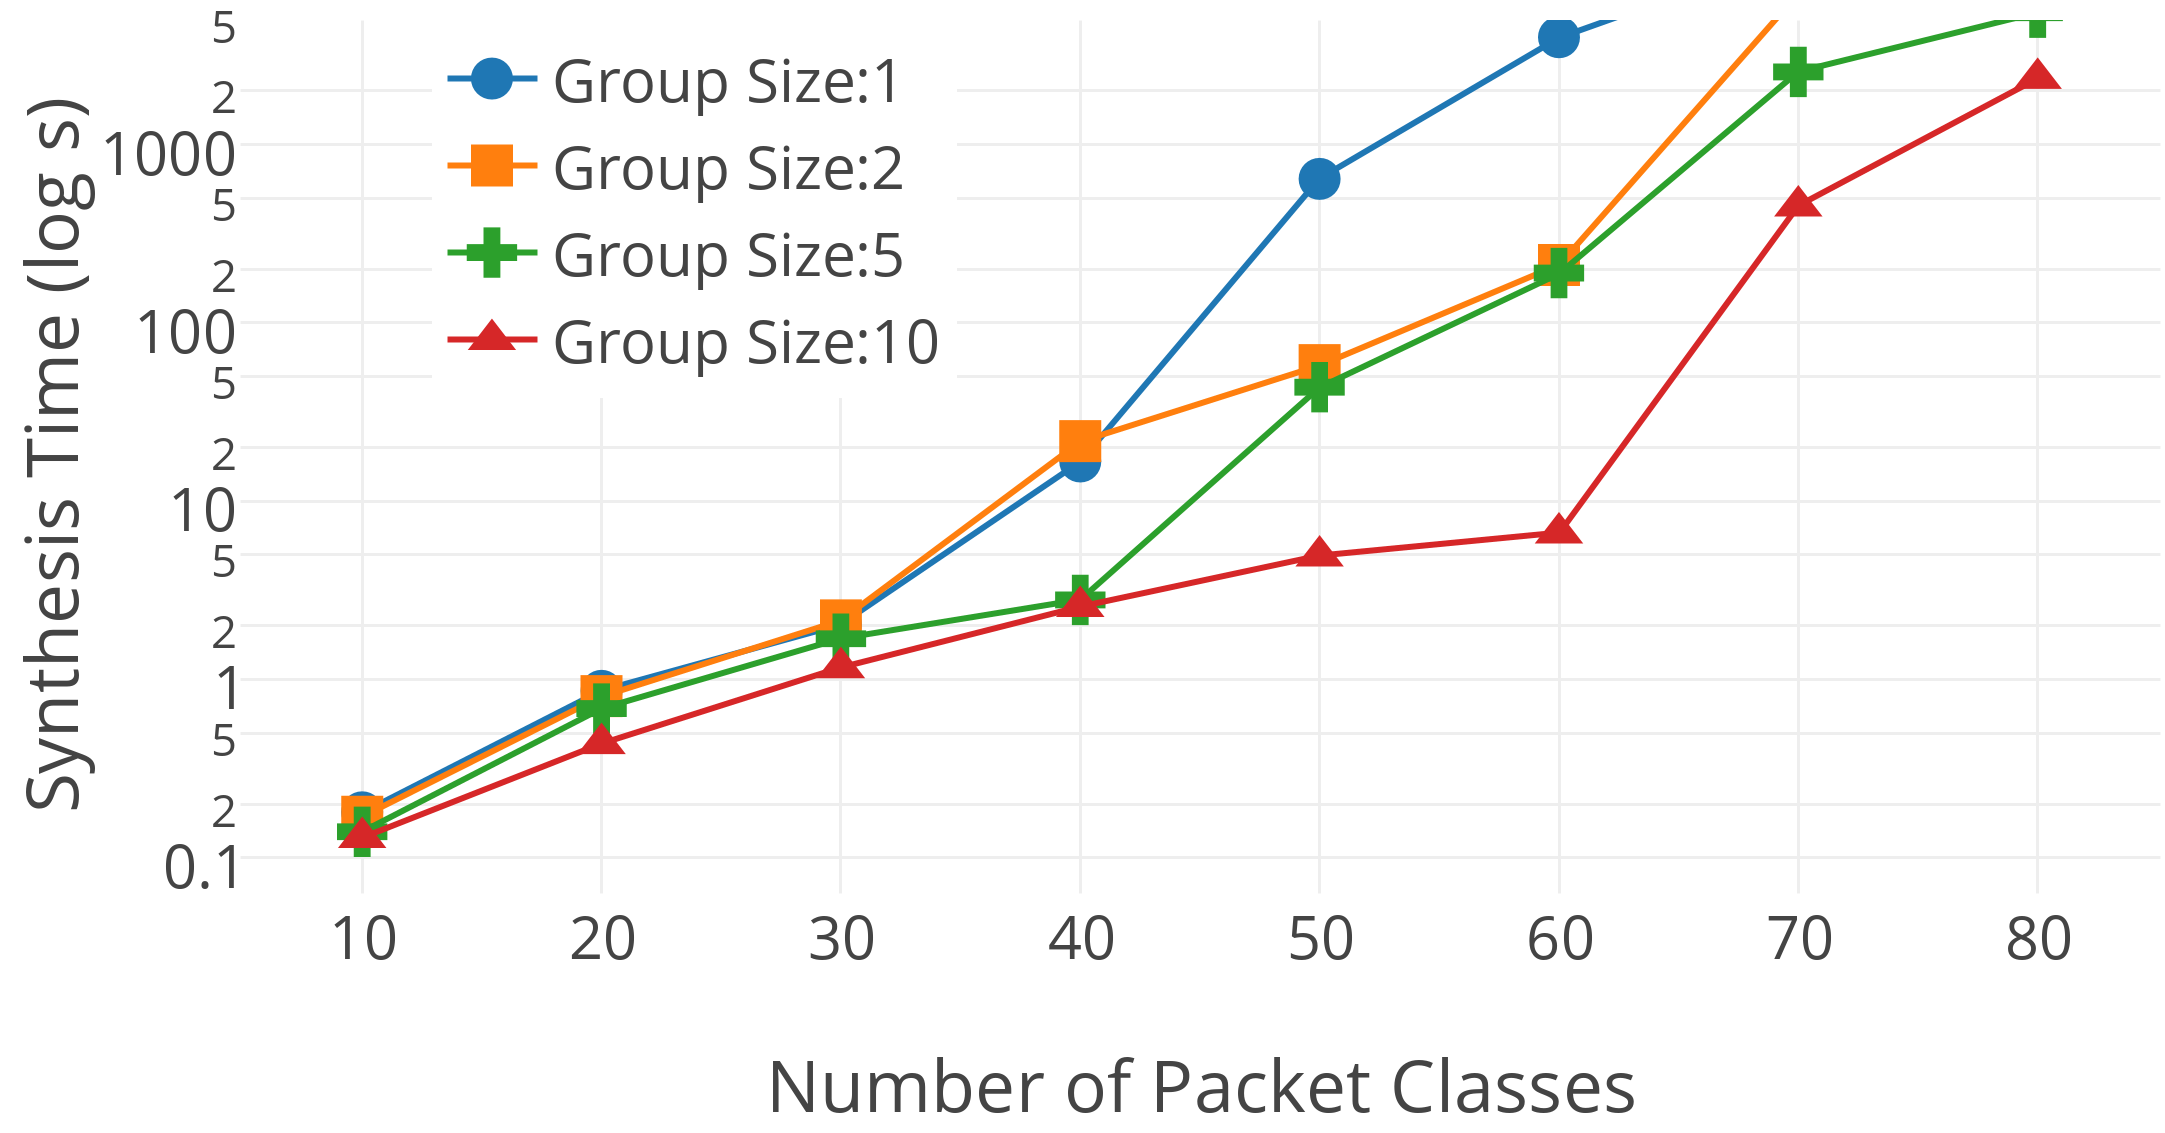
\includegraphics[width=\columnwidth]{figures/no-tactic-isolation-plot.png}
%	\caption{Synthesis time (log scale) with no tactics for range of packet classes and different tenant-group sizes.}
%	\label{fig:no-tactic}
%\end{figure}

To evaluate \Name across increasing topology sizes for isolation workloads, 
we fix the tenant-group size to 5, and for each topology, we maintain
 the ratio of packet classes to number of edge-aggregate links to 0.25. 
 We fix this metric to represent the difficulty of packing, as the maximum number 
 of different tenant sources and destination that can be present at a edge switch
 is the number of edge-aggregate links at the switch, otherwise tenant-isolation
 will be violated at the switch. If we fixed the number of packet classes, it would 
 be relatively easier to enforce policies in bigger topologies due to increasing 
 number of links. The average synthesis time per class for
 on increasing fat-tree topology sizes is shown in \cref{fig:no-tactic-topo}. 
 We are able to synthesize 12 tenants with tenant-group size 5 in a 125-node topology in 124 seconds. 
  We can also observe that average time per flow increases expotential 
  with increasing topology, thus the synthesis problem is expotential with number of nodes as well. 
		

\subsection{Tactic Reductions}
Performance of \Name for isolation workloads using normal synthesis are not 
very promising, due to the large solution space of forwarding plane configurations. We 
demonstrate the improvements of using tactics for different tenants and group sizes on a 
80-node fat-tree topology.
\Cref{fig:isolation}(b) shows the synthesis time for isolation workloads using the no edge tactic 
($\neg(e .^* e .^* e)$). We achieve a best-case speedup of 9.5x over normal synthesis with this tactic. 
Using this tactic, we are able to synthesize 12 tenants with group size in under 200
seconds.

For the same isolation workloads as above, we use the tactic $\neg (e .^5 .^* e)$ $\wedge \neg (e .^* e .^* e)$
which ensures {\em valley-free routing}, that is paths are of the form $eacae$. 
The results are shown in \cref{fig:isolation}(c). 
While this is a highly
restrictive tactic, we were able to synthesize the forwarding rules for each workload in under 20 seconds, 
and can achieve a best-case reduction of 400x compared to synthesis with no tactics. In \cref{fig:tactic-topo},
we evaluate the performance of different tactics for different topology sizes. Tactics can provide 
a considerable improvement over the baseline performance as illustrated by these experiments. 

\subsection{Optimistic Synthesis Performance}
To evaluate the heuristical optimistic synthesis procedure, we perform 100 runs of normal and optimistic synthesis (with the "no edge" tactic) to isolation
 workloads with varying number of tenants and different group sizes 
we used in the \cref{fig:isolation} experiment and computed the
 speedup $t(Optimistic)/$ $t(normal)$ and plotted its cumulative frequency
  distribution as shown in \cref{fig:opt-cdf}. For more than 80\% of the
workloads, optimistic gets a better or comparable performance to normal synthesis, with
achieving a speedup of 2X nearly 40\% of the workloads. For 20\% of the workloads, optimistic
performs worse than normal, especially for group size 1 workloads.

\subsection{Incremental Synthesis Performance}
While network management systems have support for enforcing complex policies, 
a important feature required from these systems is to be enforce incremental changes
like addition of new tenants, changes to policies or topology events like link/switch 
failures. To evaluate our synthesis algorithm for incremental changes, we use 100 runs of 
different isolation workloads of the \cref{fig:isolation} experiment and perform synthesis, and then
add a single policy to a tenant (with isolation policies to all other tenant packet classes) and
measure the time needed for synthesis of the updated policies. We plot a cumulative frequency 
distribution of the ratio of time taken for incremental synthesis versus the time taken for normal 
"one-shot" synthesis in \cref{fig:incremental-cdf}. For 80 \% of the workloads, the incremental 
synthesis takes less than 10\% of the normal synthesis time which makes \Name suitable for 
performing incremental changes, but in some cases, the new policies may trigger a re-synthesis 
of the previously synthesized policies, and we can see workloads where the ratio is close to 1. 
Thus, solving incremental synthesis is a challenging problem and is one of the future directions
to building a robust network management system. 

%\begin{figure*}
%	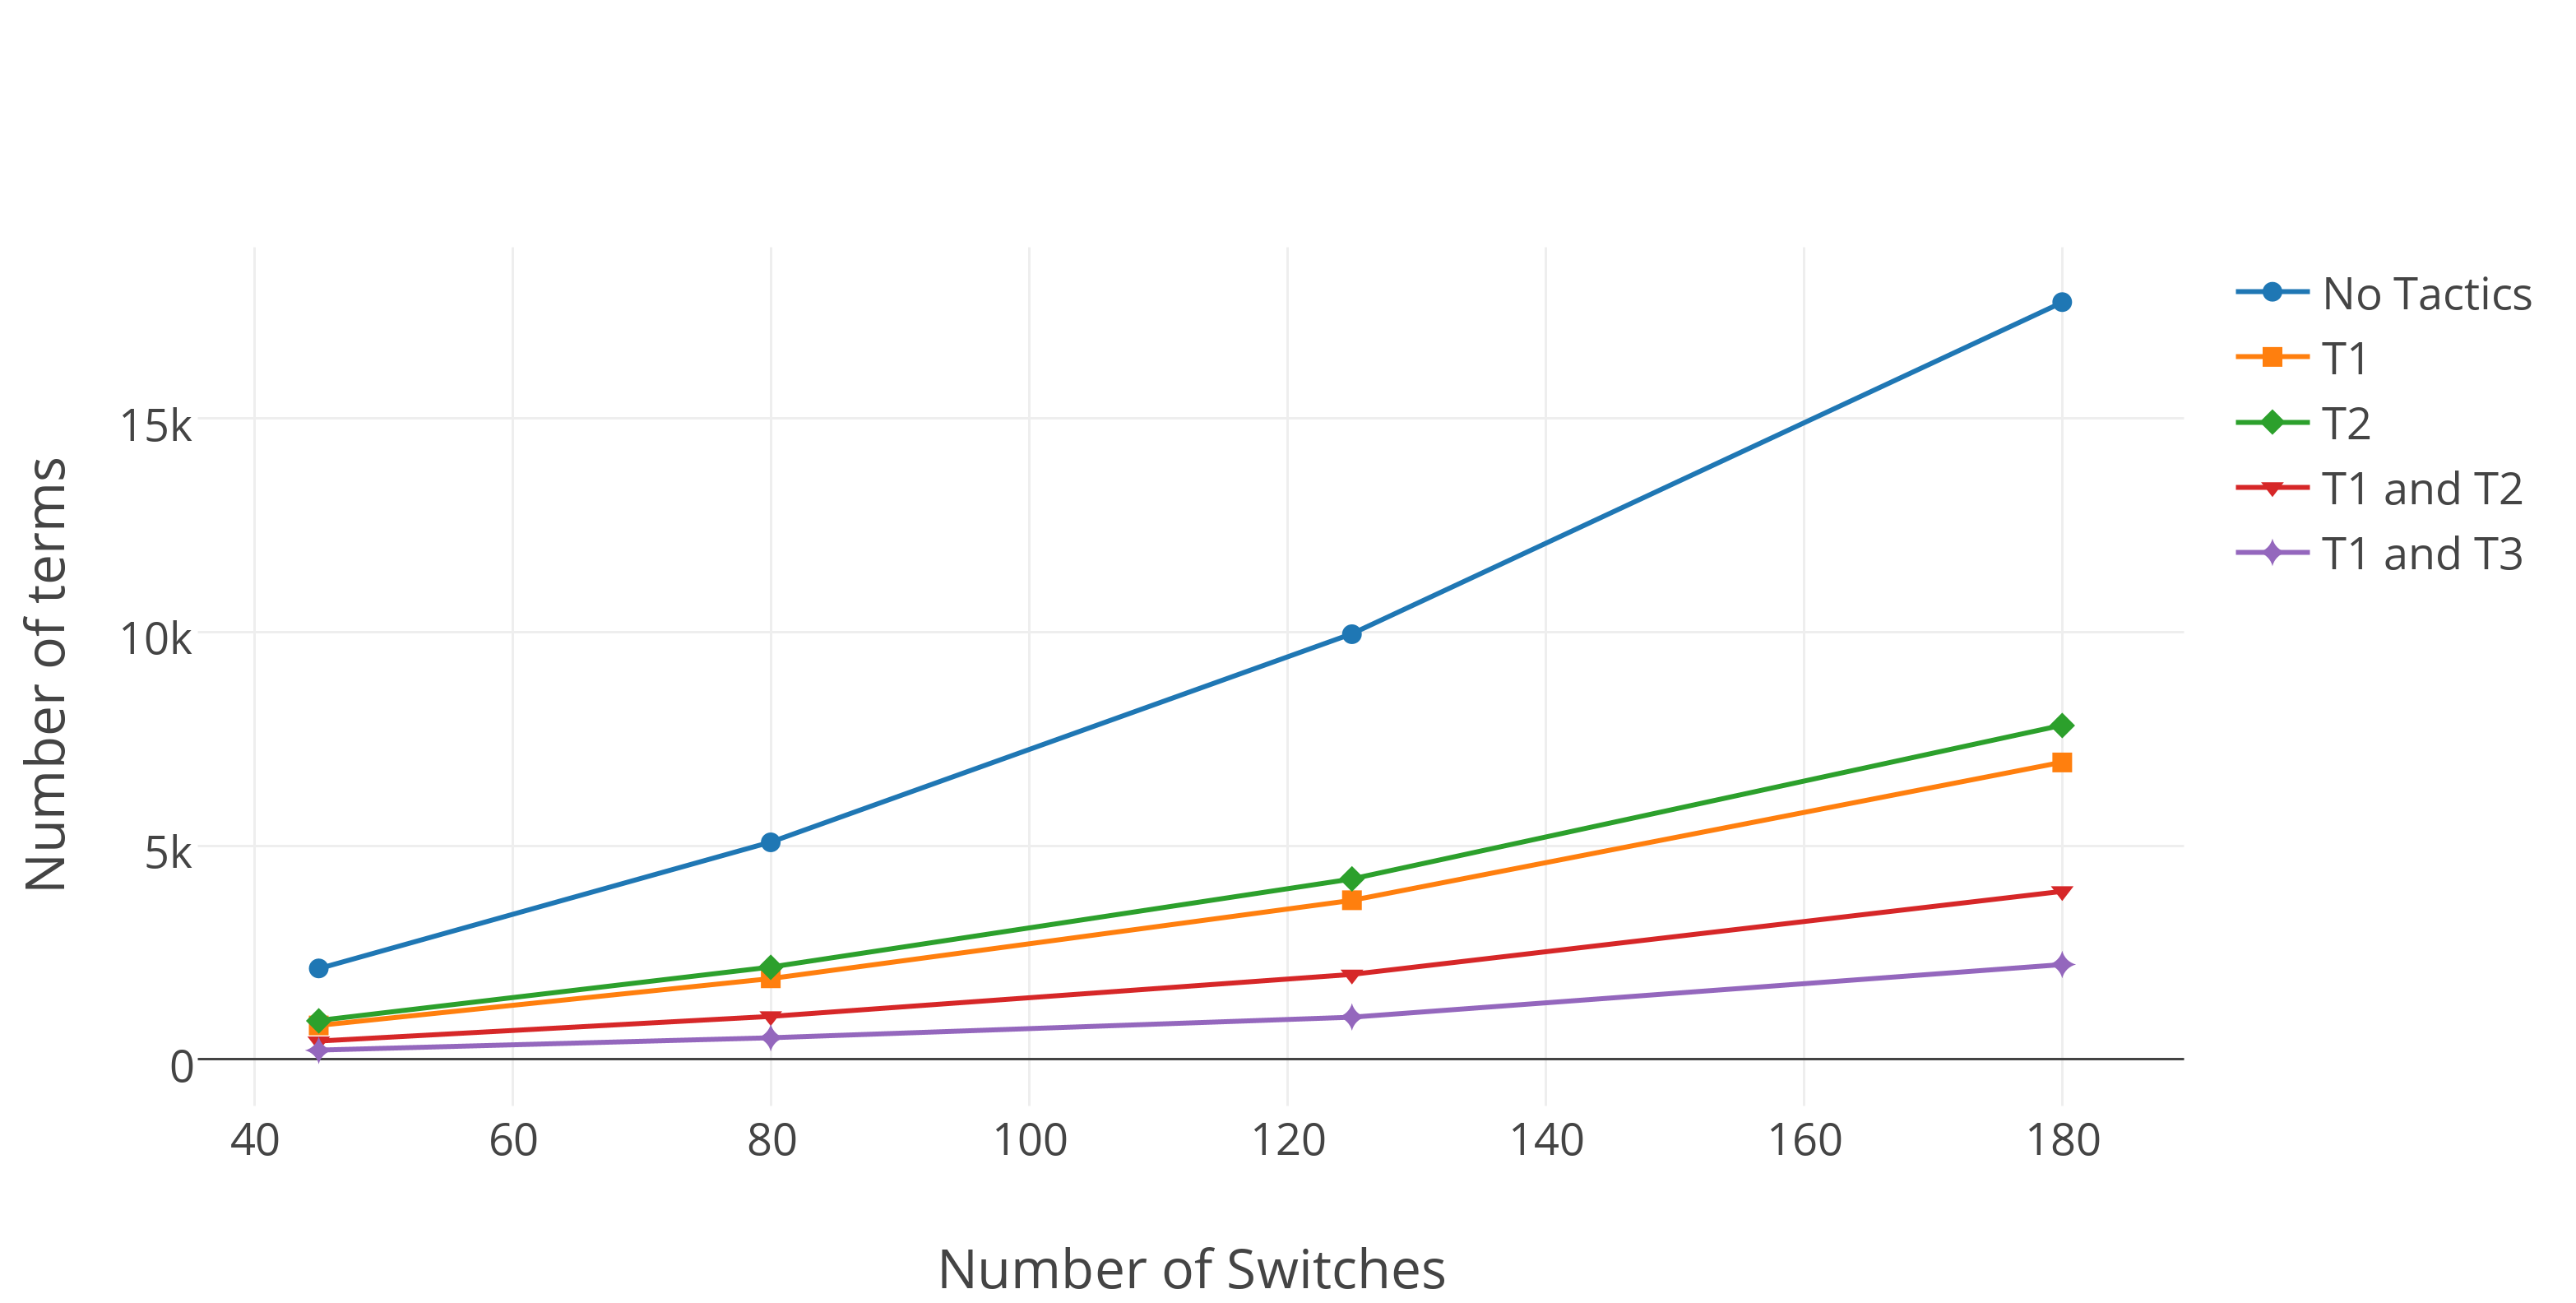
\includegraphics[height=7.5cm]{figures/tactic-reduction.png}
%	\caption{Graph used to show the reduction of terms using different tactics w.r.t the total number of terms}
%	\label{fig:tactic-reduction}
%\end{figure*}
%
%\begin{figure}
%	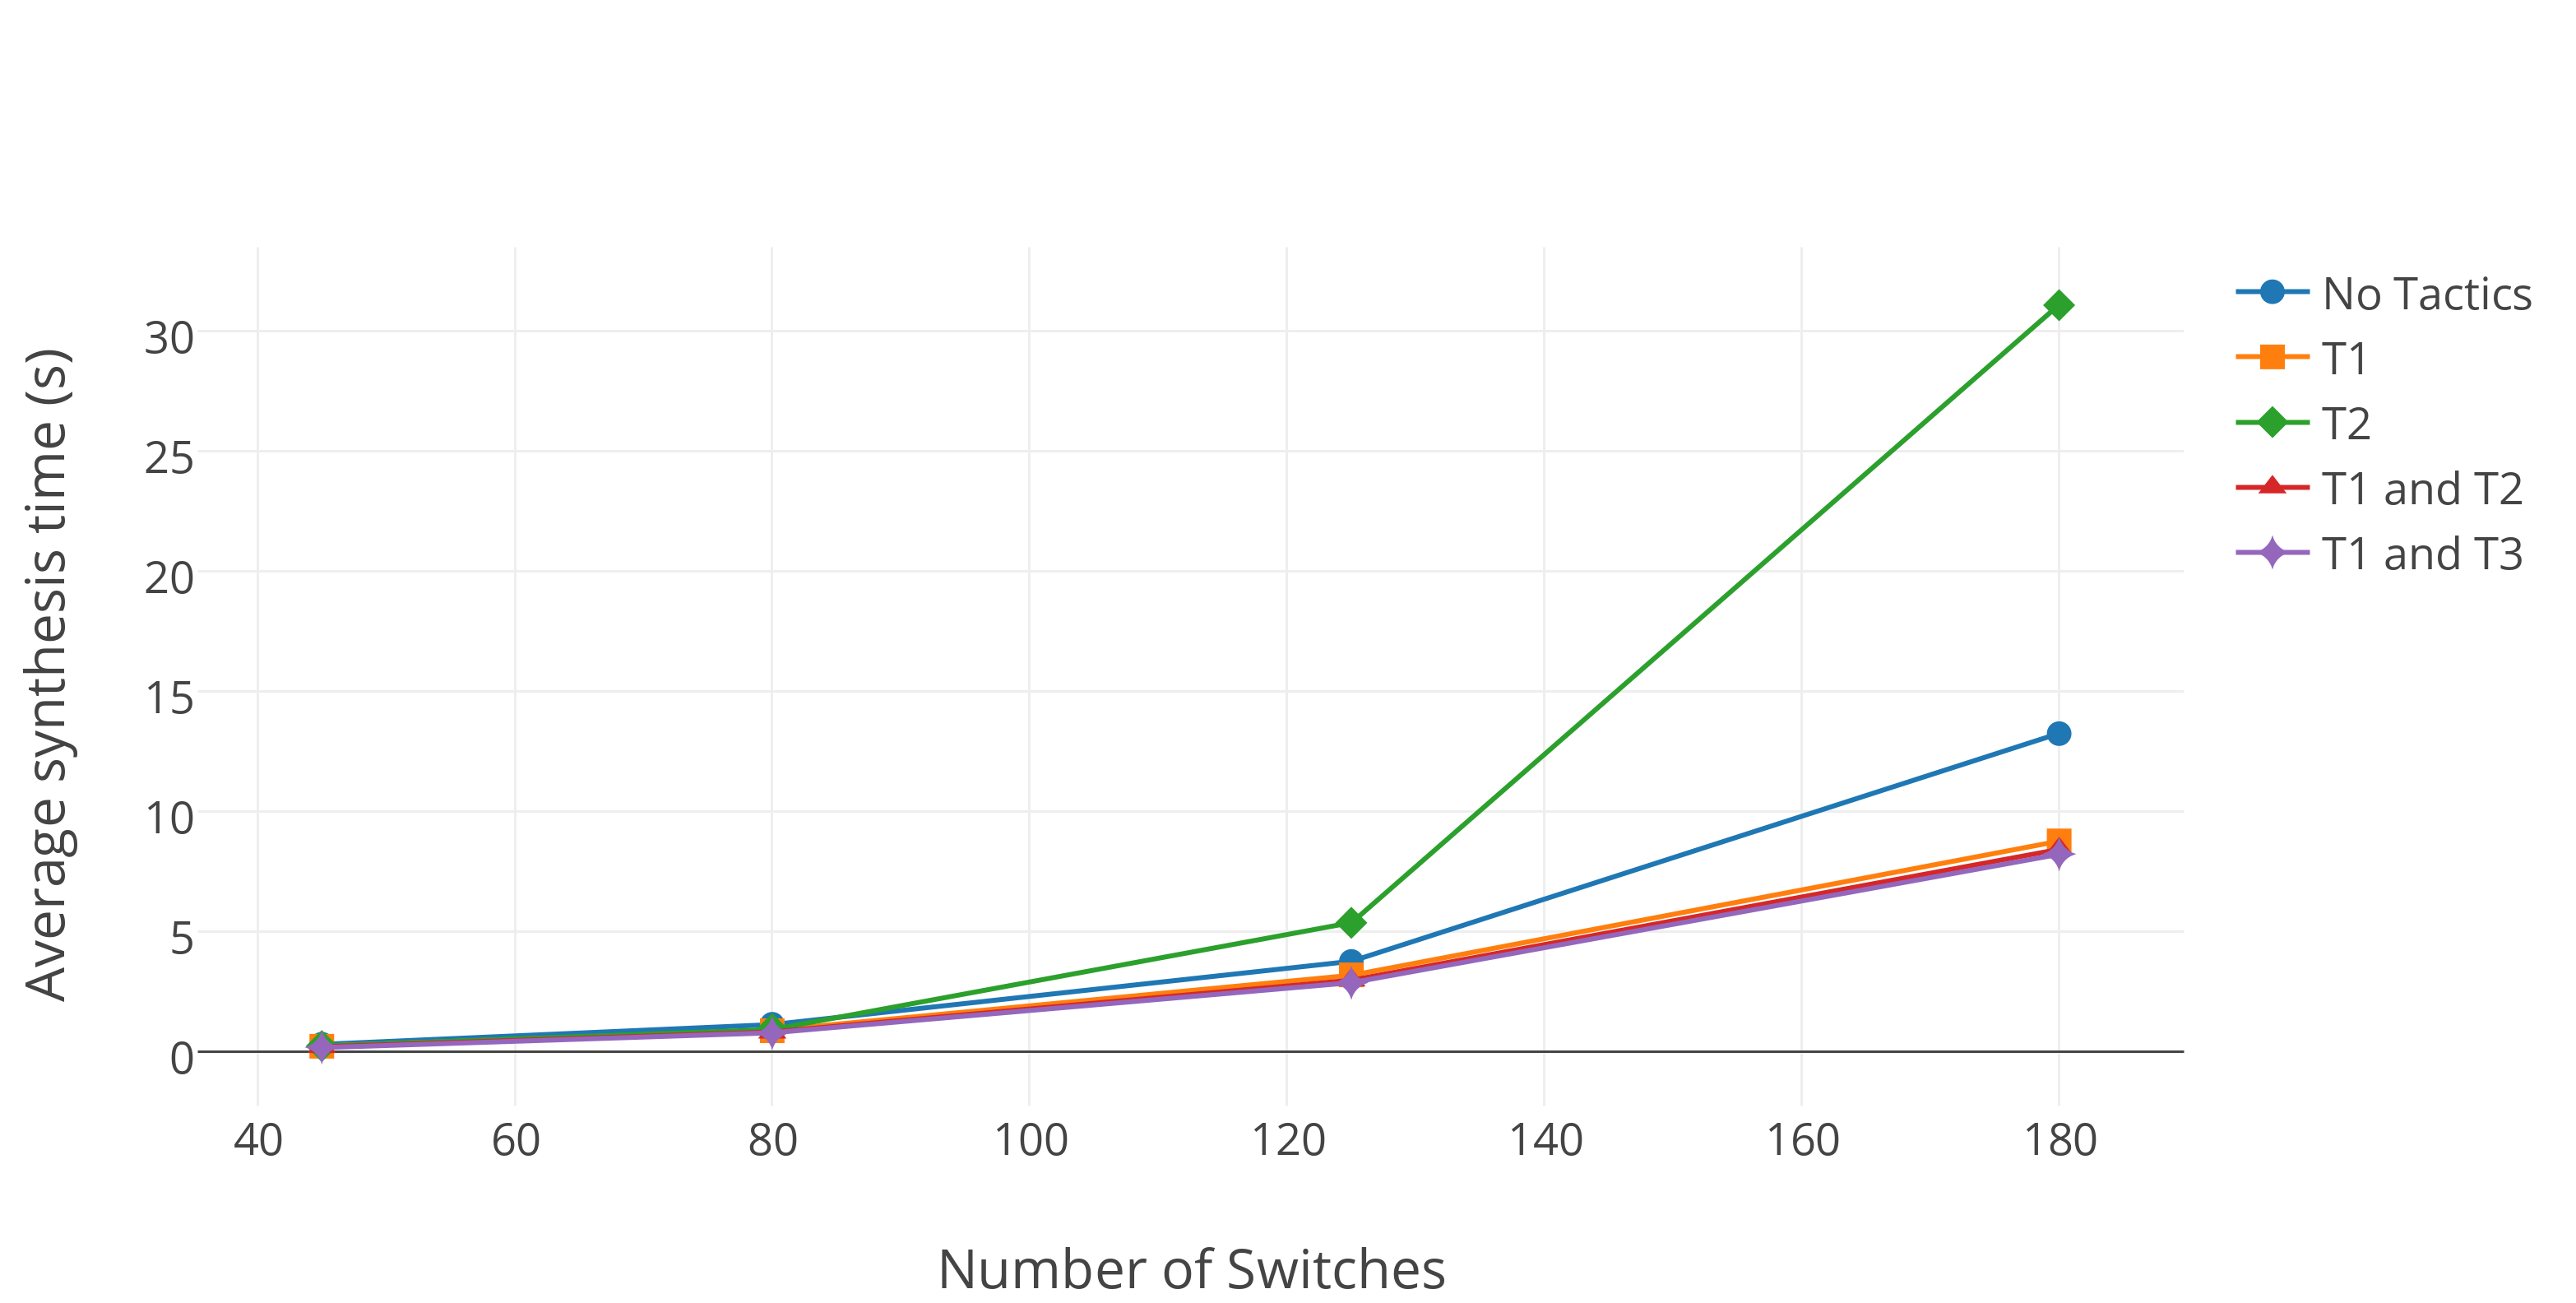
\includegraphics[width=\columnwidth]{figures/isolation-tactics.png}
%	\caption{Graph used to application of tactics for a isolation workload (percentage isolation w.r.t topology 25\%) and different topology sizes. An interesting observation in the graph is that tactics need not always help in reduction of constraints (One of the tactics, not  a very natural one) leads to more time to synthesis without tactics.}
%	\label{fig:isolation-tactics}
%\end{figure}
%
%\subsection{Optimistic Synthesis}
\begin{figure}
	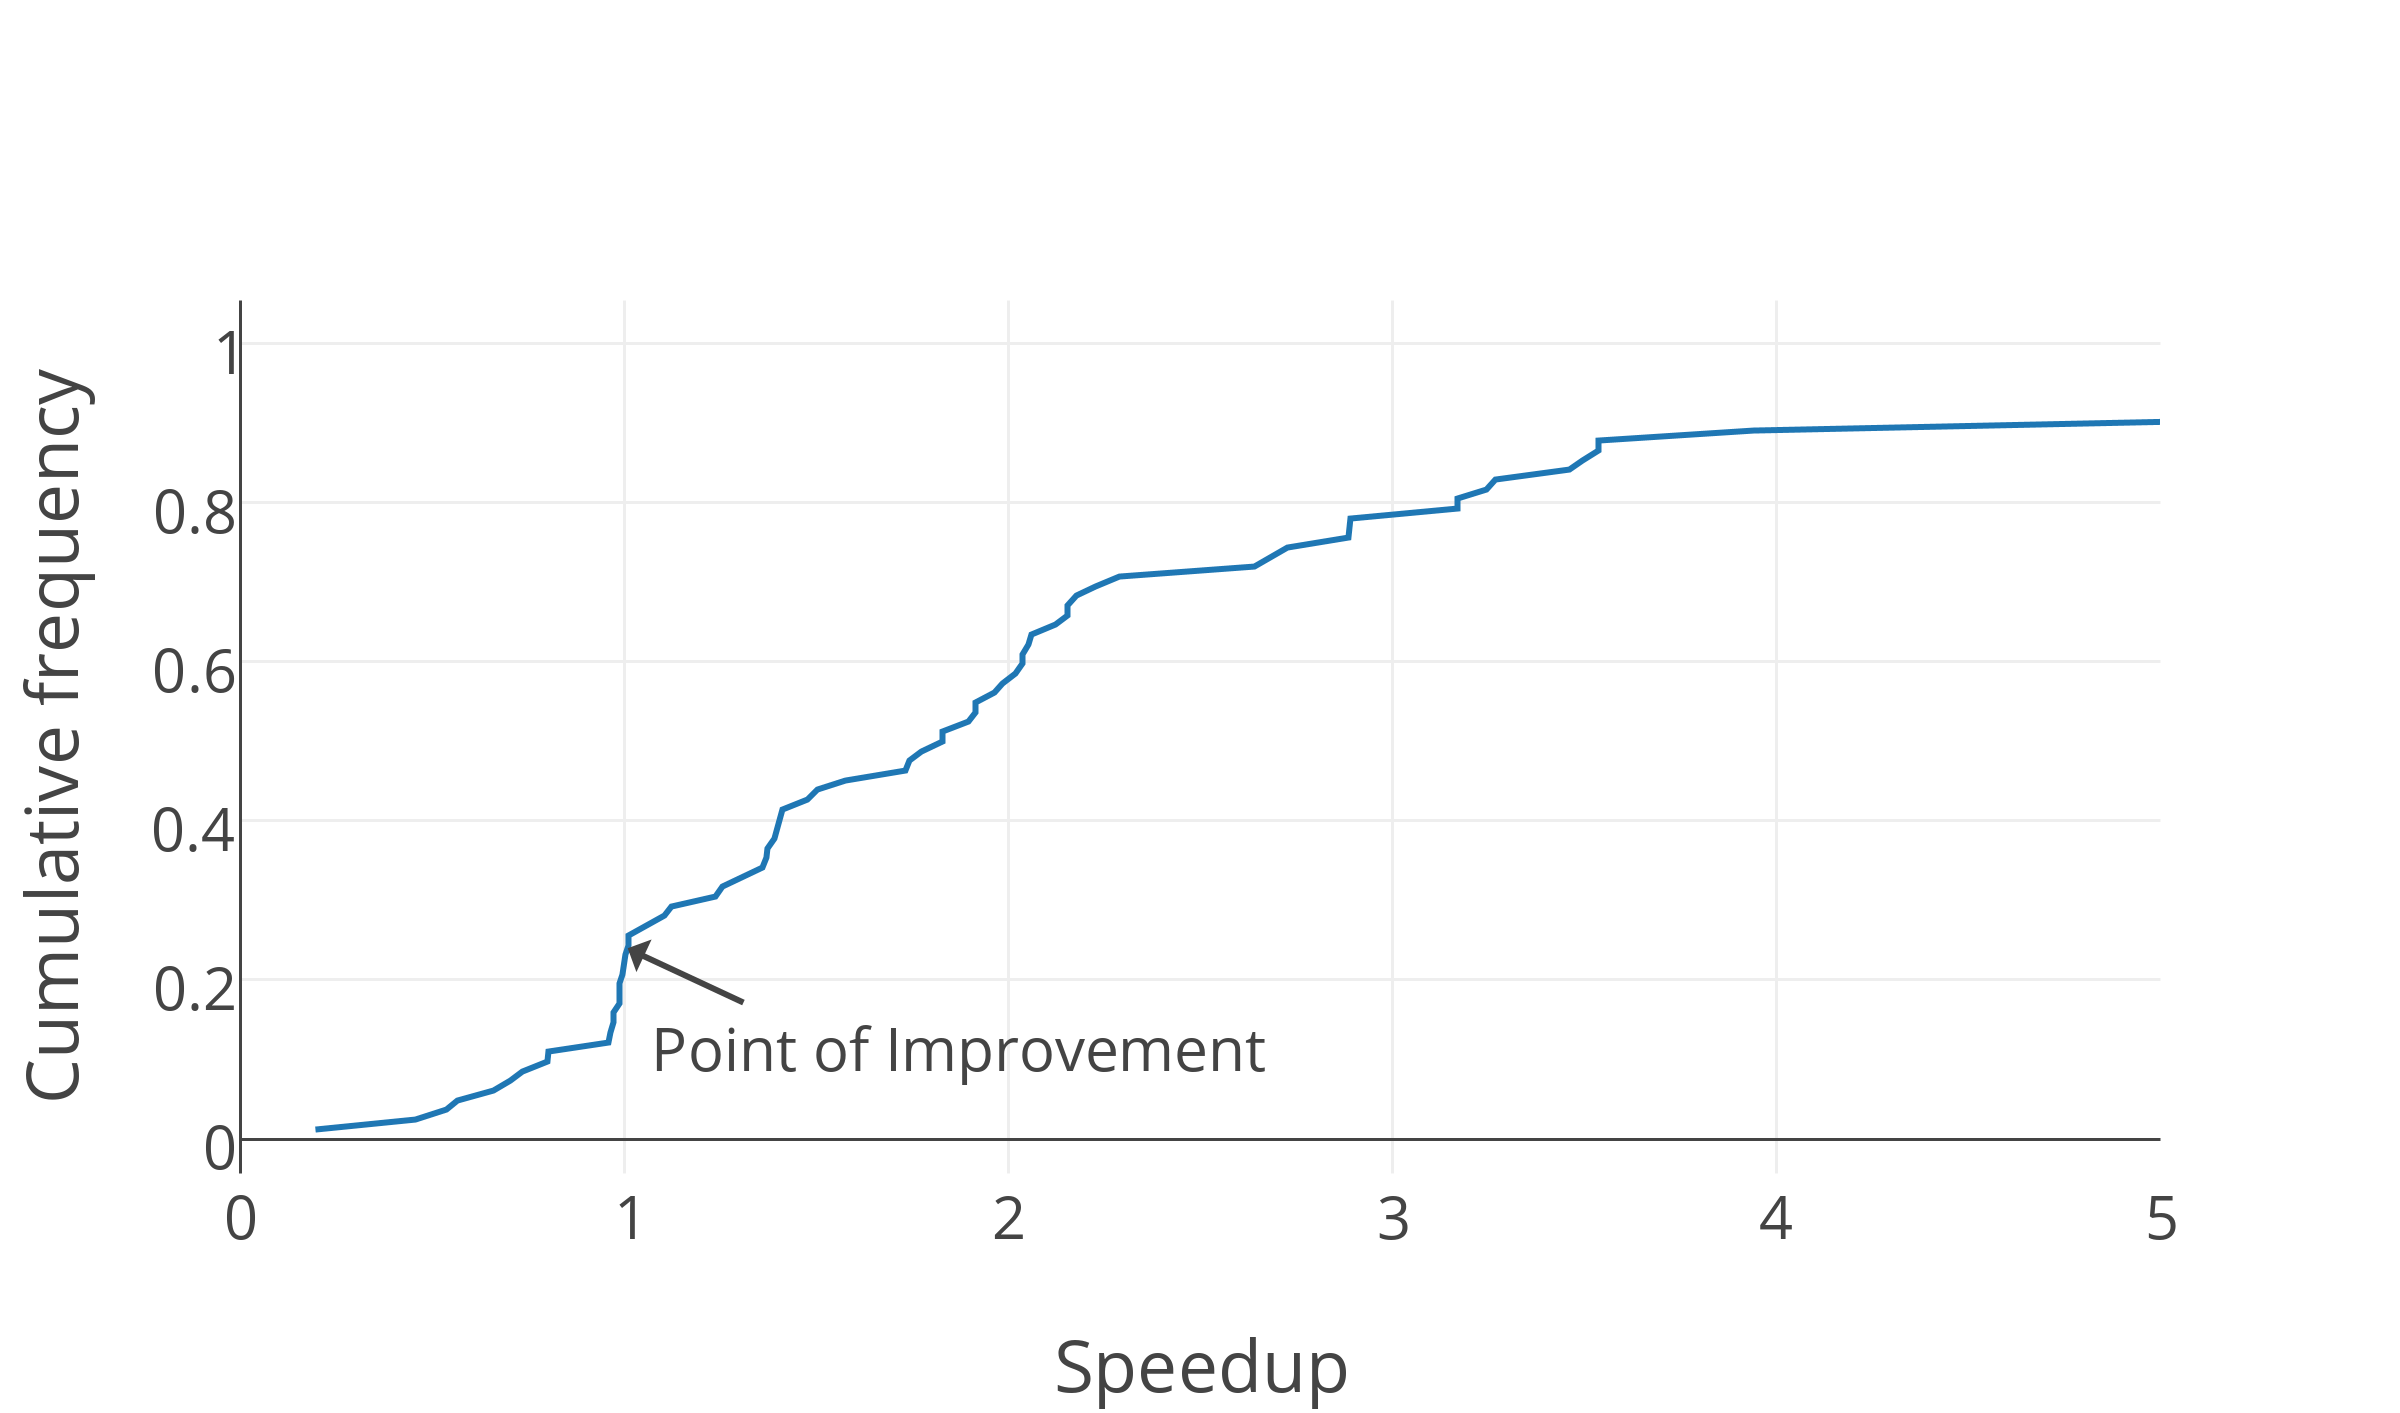
\includegraphics[width=\columnwidth]{figures/opt-cdf.eps}
	\caption{Cumulative frequency distribution for speedup achieved by optimistic synthesis.}
	\label{fig:opt-cdf}
\end{figure}
\begin{figure}
	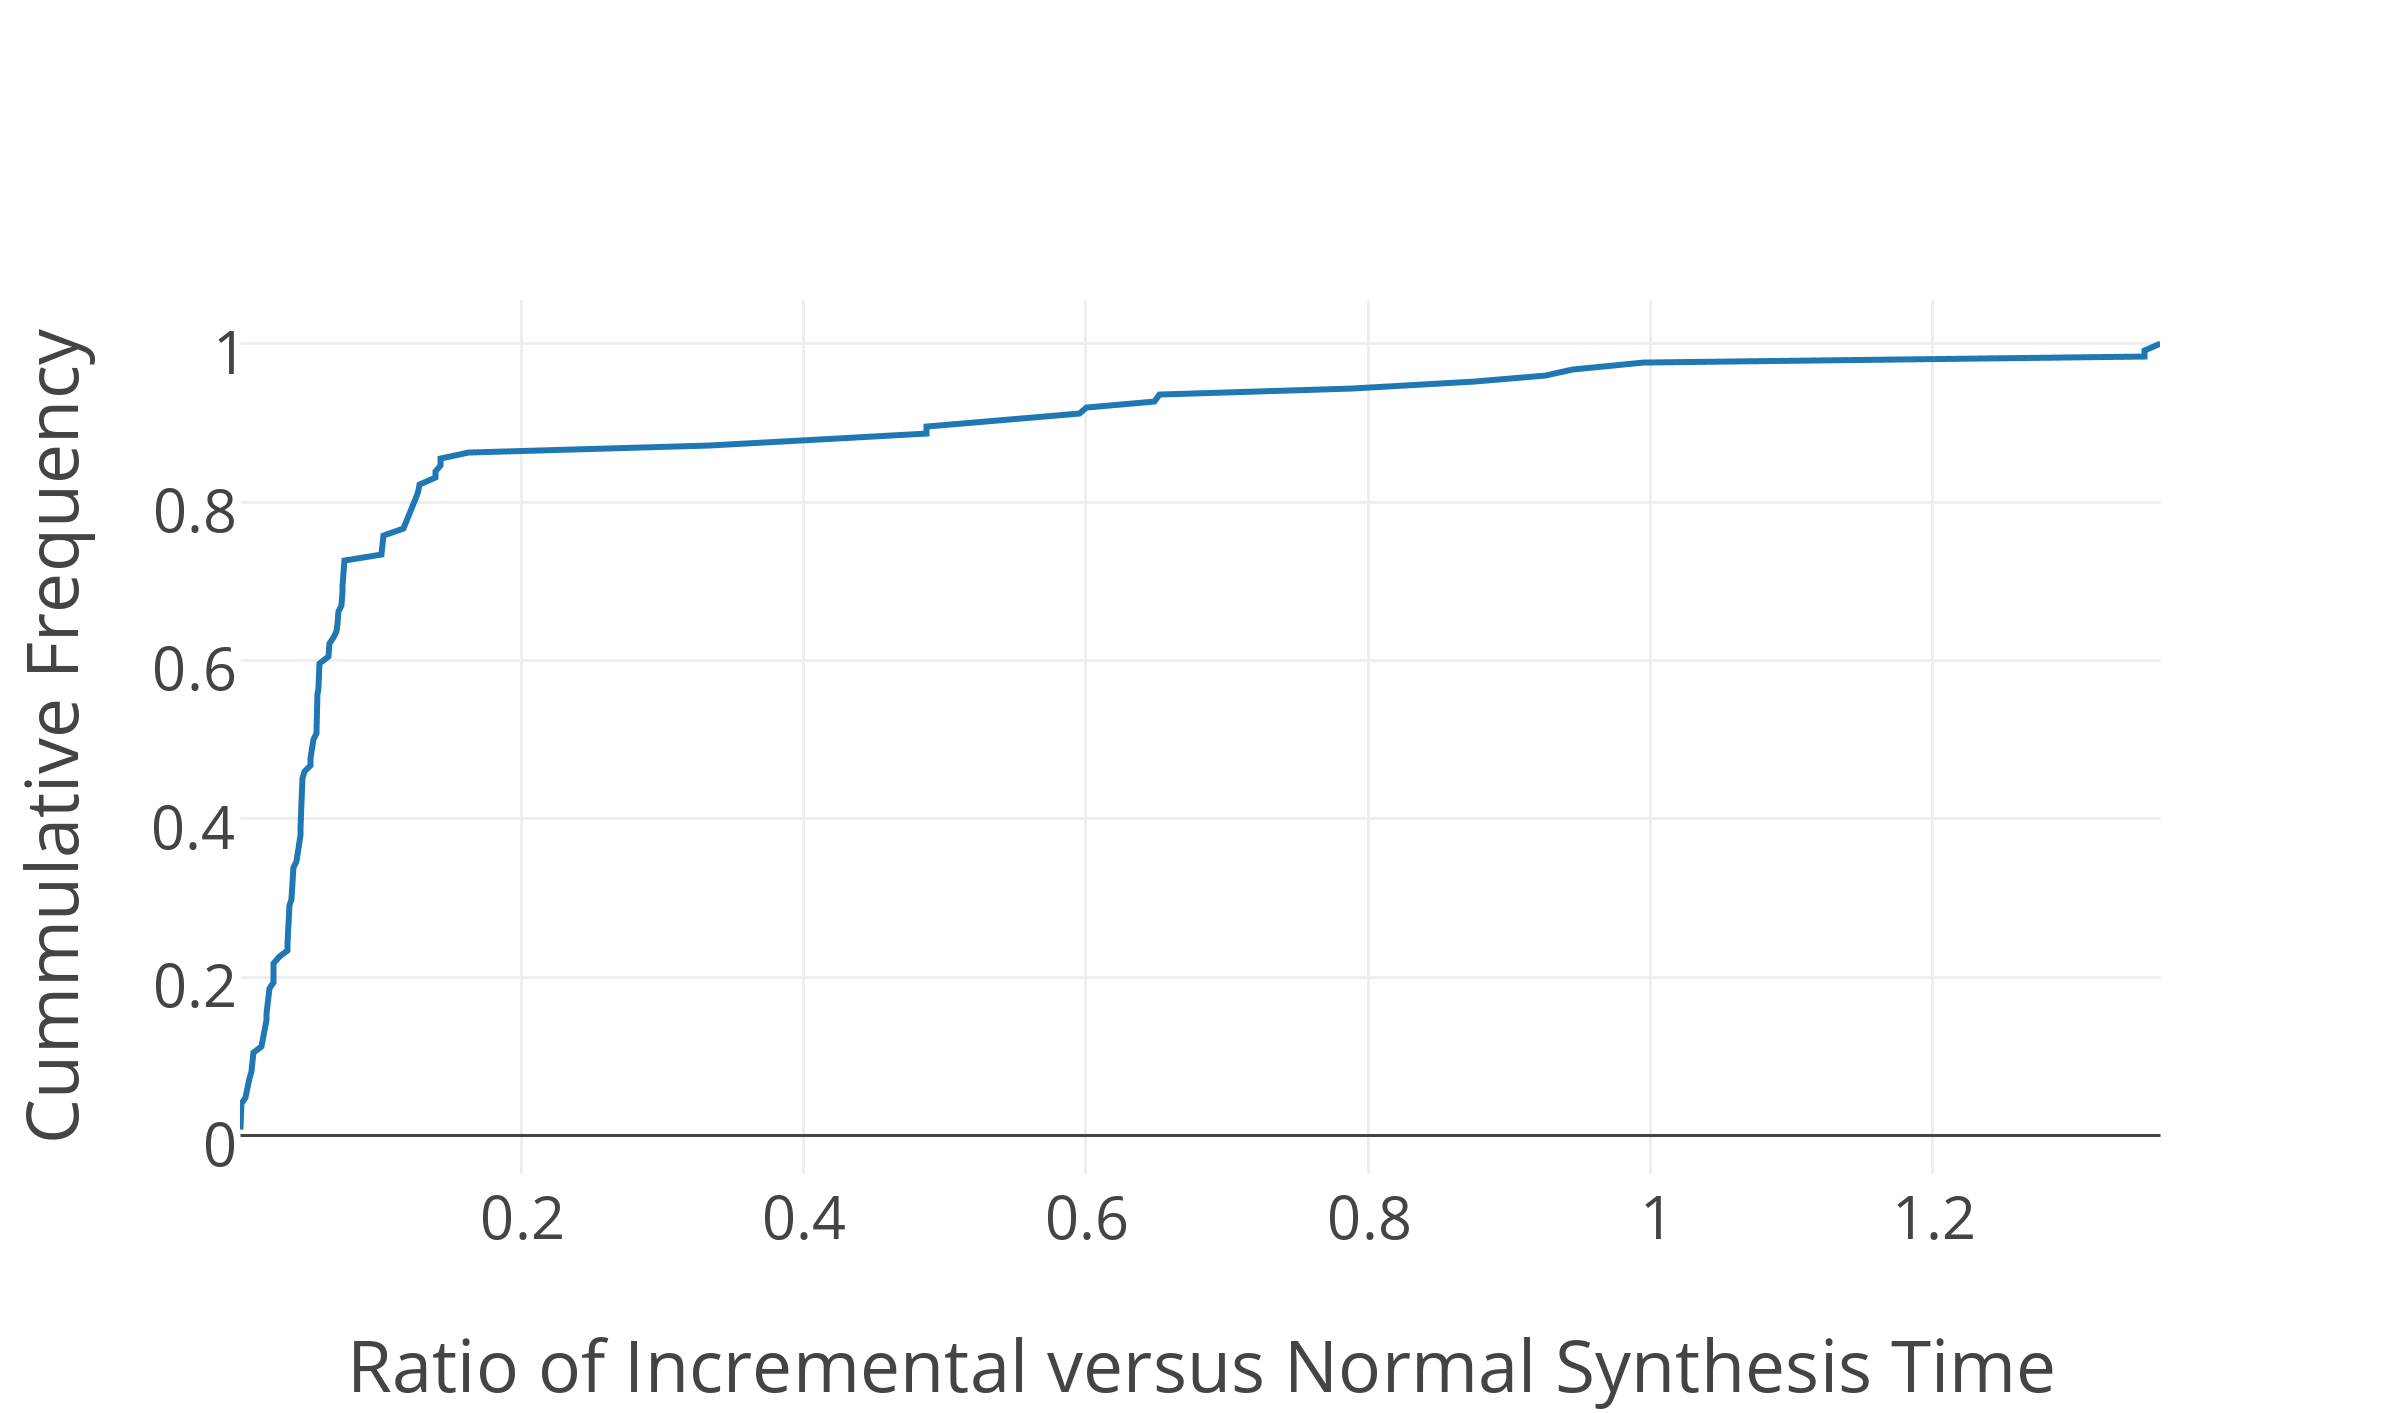
\includegraphics[width=\columnwidth]{figures/incremental-cdf.eps}
	\caption{Cumulative frequency distribution for ratio of incremental synthesis/one-shot synthesis.}
	\label{fig:incremental-cdf}
\end{figure}


%\caption{Synthesis Time for varying number of reachability (with and without tactics) and waypoints policies for a 45 node fat-tree topology}


